\documentclass[addpoints, 12pt]{exam}%, answers]
\usepackage[utf8]{inputenc}
\usepackage[T1]{fontenc}

\usepackage{lmodern}
\usepackage{arydshln}
\usepackage[margin=2cm]{geometry}

\usepackage{enumitem}

\usepackage{amsmath, amsthm, amsfonts, amssymb}
\usepackage{graphicx}
\usepackage{tikz}
\usetikzlibrary{arrows,calc,patterns}
\usepackage{pgfplots}
\pgfplotsset{compat=newest}
\usepackage{url}
\usepackage{multicol}
\usepackage{thmtools}
\usepackage{wrapfig}

\usepackage{caption}
\usepackage{subcaption}

\usepackage{pifont}

% MATH commands
\newcommand{\bC}{\mathbb{C}}
\newcommand{\bR}{\mathbb{R}}
\newcommand{\bN}{\mathbb{N}}
\newcommand{\bZ}{\mathbb{Z}}
\newcommand{\bT}{\mathbb{T}}
\newcommand{\bD}{\mathbb{D}}

\newcommand{\cL}{\mathcal{L}}
\newcommand{\cM}{\mathcal{M}}
\newcommand{\cP}{\mathcal{P}}
\newcommand{\cH}{\mathcal{H}}
\newcommand{\cB}{\mathcal{B}}
\newcommand{\cK}{\mathcal{K}}
\newcommand{\cJ}{\mathcal{J}}
\newcommand{\cU}{\mathcal{U}}
\newcommand{\cO}{\mathcal{O}}
\newcommand{\cA}{\mathcal{A}}
\newcommand{\cC}{\mathcal{C}}
\newcommand{\cF}{\mathcal{F}}

\newcommand{\fK}{\mathfrak{K}}
\newcommand{\fM}{\mathfrak{M}}

\newcommand{\ga}{\left\langle}
\newcommand{\da}{\right\rangle}
\newcommand{\oa}{\left\lbrace}
\newcommand{\fa}{\right\rbrace}
\newcommand{\oc}{\left[}
\newcommand{\fc}{\right]}
\newcommand{\op}{\left(}
\newcommand{\fp}{\right)}

\newcommand{\ra}{\rightarrow}
\newcommand{\Ra}{\Rightarrow}

\renewcommand{\Re}{\mathrm{Re}\,}
\renewcommand{\Im}{\mathrm{Im}\,}
\newcommand{\Arg}{\mathrm{Arg}\,}
\newcommand{\Arctan}{\mathrm{Arctan}\,}
\newcommand{\sech}{\mathrm{sech}\,}
\newcommand{\csch}{\mathrm{csch}\,}
\newcommand{\Log}{\mathrm{Log}\,}
\newcommand{\cis}{\mathrm{cis}\,}

\newcommand{\ran}{\mathrm{ran}\,}
\newcommand{\bi}{\mathbf{i}}
\newcommand{\Sp}{\mathrm{span}\,}
\newcommand{\Inv}{\mathrm{Inv}\,}
\newcommand\smallO{
  \mathchoice
    {{\scriptstyle\mathcal{O}}}% \displaystyle
    {{\scriptstyle\mathcal{O}}}% \textstyle
    {{\scriptscriptstyle\mathcal{O}}}% \scriptstyle
    {\scalebox{.7}{$\scriptscriptstyle\mathcal{O}$}}%\scriptscriptstyle
  }
\newcommand{\HOL}{\mathrm{Hol}}
\newcommand{\cl}{\mathrm{clos}}
\newcommand{\ve}{\varepsilon}

\DeclareMathOperator{\dom}{dom}

%%%%%% Définitions Theorems and al.
%\declaretheoremstyle[preheadhook = {\vskip0.2cm}, mdframed = {linewidth = 2pt, backgroundcolor = yellow}]{myThmstyle}
%\declaretheoremstyle[preheadhook = {\vskip0.2cm}, postfoothook = {\vskip0.2cm}, mdframed = {linewidth = 1.5pt, backgroundcolor=green}]{myDefstyle}
%\declaretheoremstyle[bodyfont = \normalfont , spaceabove = 0.1cm , spacebelow = 0.25cm, qed = $\blacktriangle$]{myRemstyle}

%\declaretheorem[ style = myThmstyle, name=Th\'eor\`eme]{theorem}
%\declaretheorem[style =myThmstyle, name=Proposition]{proposition}
%\declaretheorem[style = myThmstyle, name = Corollaire]{corollary}
%\declaretheorem[style = myThmstyle, name = Lemme]{lemma}
%\declaretheorem[style = myThmstyle, name = Conjecture]{conjecture}

%\declaretheorem[style = myDefstyle, name = D\'efinition]{definition}

%\declaretheorem[style = myRemstyle, name = Remarque]{remark}
%\declaretheorem[style = myRemstyle, name = Remarques]{remarks}

\newtheorem{theorem}{Théorème}
\newtheorem{corollary}{Corollaire}
\newtheorem{lemma}{Lemme}
\newtheorem{proposition}{Proposition}
\newtheorem{conjecture}{Conjecture}

\theoremstyle{definition}

\newtheorem{definition}{Définition}[section]
\newtheorem{example}{Exemple}[section]
\newtheorem{remark}{\textcolor{red}{Remarque}}[section]
\newtheorem{exer}{\textbf{Exercice}}[section]


\tikzstyle{myboxT} = [draw=black, fill=black!0,line width = 1pt,
    rectangle, rounded corners = 0pt, inner sep=8pt, inner ysep=8pt]

\begin{document}
	\noindent \hrulefill \\
	\noindent MATH-241 \hfill Created by Pierre-O. Paris{\'e}\\
	Midterm 01 \hfill 2023/22/02, Spring 2023\\\vspace*{-0.7cm}

\noindent\hrulefill
	
\vspace*{1cm}

\noindent\makebox[\textwidth]{\textbf{Last name:}\enspace \hrulefill}

\vspace*{0.5cm}

\noindent\makebox[\textwidth]{\textbf{First name:}\enspace\hrulefill}

\vspace*{0.5cm}

\noindent\makebox[\textwidth]{\textbf{Section:}\enspace\hrulefill}

\vspace*{1cm}

\noindent\textbf{Instructions:} 

\begin{itemize}
\item Make sure to write your complete name on your copy. 
\item You must answer all eight (8) questions below and write your answers directly on the questionnaire.
\item You have 75 minutes to complete the exam.
\item When you are done (or at the end of the 75min period), return your copy. 
\item Devices such as smartphones, cellphones, laptops, tablets, e-readers, ipods, gameboys (and, you know, any other electronic devices that I haven't thought of) may not be used during the exam. 
\item You can not use a calculator.
\item \textbf{Turn off your cellphones during the exam}.
\item Lecture notes and the textbook are not allowed during the exam. 
\item You must show ALL your work to have full credit. An answer without justification is worth no points (except if it is mentioned explicitly in the question not to justify).
\item Draw a square around your final answer.
\end{itemize}

\vspace{1cm}

\noindent\textbf{Your Signature:} \hrulefill

\vspace*{1.5cm}
\noindent \textsc{May the Force be with you!} \hfill \textsc{Pierre Parisé}

\vspace*{0.5cm}

\begin{center}
\begin{minipage}{0.29\textwidth}
\begin{Huge}
\textsc{University of Hawai'i}
\end{Huge}
\end{minipage}
\begin{minipage}{0.12\textwidth}
\includegraphics[scale=0.05]{../../../../manoaseal_transparent.png}
\end{minipage}
\end{center}

\qformat{\rule{0.3\textwidth}{.4pt} \begin{large}{\textsc{Question}} \thequestion \end{large} \hspace*{0.2cm} \hrulefill \hspace*{0.1cm} \textbf{(\totalpoints\hspace*{0.1cm} pts)}}

\vspace*{0.5cm}

\newpage % End of cover page


	
%	PLAN:

\begin{questions}
	
	\question
	The table shows the distance travelled by a bicyclist on a straight line after accelerating from rest.
	
	\begin{minipage}{0.45\textwidth}
		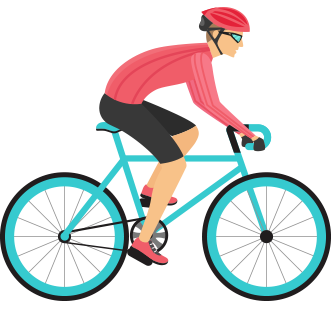
\includegraphics[width=4cm]{bic1}
	\end{minipage}
	\begin{minipage}{0.45\textwidth}
		\begin{tabular}{c|c}
			Time in seconds & Total distance in feet \\ \hline
			0 & 0 \\
			1 & 2 \\
			2 & 4 \\
			3 & 8 \\
			4 & 15 \\
			5 & 30 \\
			6 & 52 \\
			7 & 76 \\
			8 & 101	
		\end{tabular}
	\end{minipage}
	
	\phantom{2}
	
	\begin{parts}
		\part[2]
		Calculate the average speed between 2 and 6 seconds.
		\vfill
		\part[3]
		Compare the average speed of the interval between 0 second and 1 second, and the interval between 1 second and 2 seconds. Between these two intervals, which one has the highest average speed?
		\vfill
		\part[3]
		Estimate the average acceleration of the bicyclist at 7 seconds.\\ (Hint: The average acceleration can be calculated using two average speeds.) 
		\vfill
	\end{parts} 
	
	\newpage
	
	\question[15] The graph of a function $f$ is given below. Assume $f$ has vertical asymptotes at $x=-1$ and $x=1$. \textbf{No justification needed for this problem.}
	
	\begin{center}
	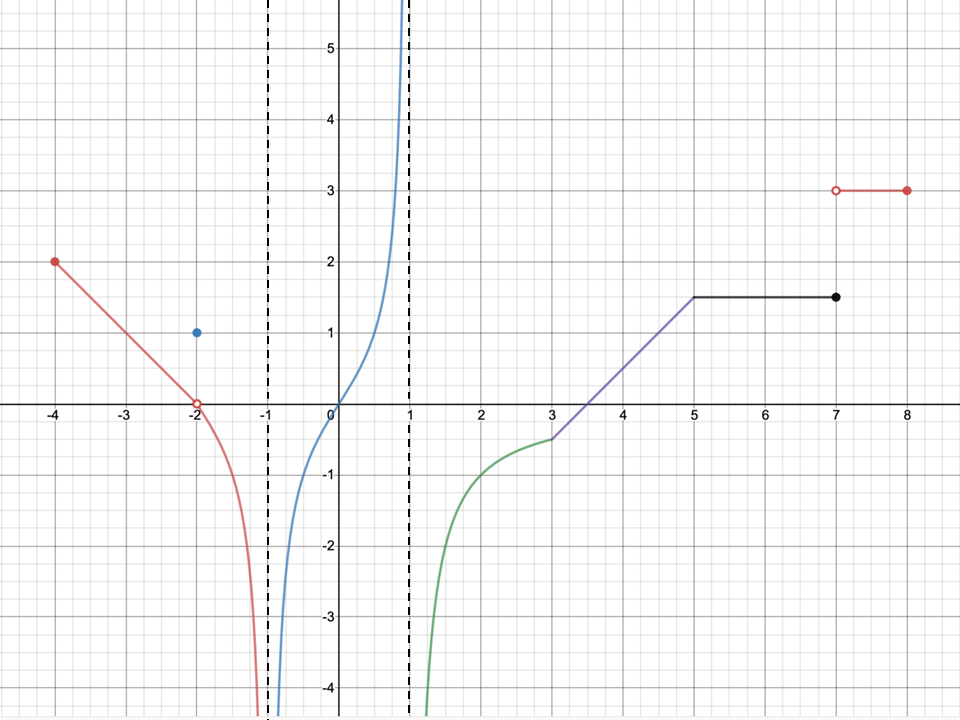
\includegraphics[width = 12cm]{graph.png}
	\end{center}
	
	\begin{parts}
		\part (6 points) Evaluate each of the following limits, or say the limit does not exist. If the limit is either $\infty$ or $-\infty$, specify which (rather than just saying `does not exist').
		\begin{enumerate}
			\begin{multicols}{2}
				\item $\displaystyle\lim_{x\to -2} f(x)$\\
				\item $\displaystyle\lim_{x\to -1^-} f(x)$\\
				\item $\displaystyle\lim_{x\to 1} f(x)$ \\
				\columnbreak
				\item $\displaystyle\lim_{x\to 7^-} f(x)$\\ 
				\item $\displaystyle\lim_{x\to 7^+} f(x)$ \\
				\item $\displaystyle\lim_{x\to 7} f(x)$ \\		
			\end{multicols}
		\end{enumerate}
		
		\part (3 points) For which (if any) values in the interval $[-4,8]$ is the function $f$ not continuous?
		\vfill
		
		\part (3 points) For which (if any) values in the interval $[-4,8]$ is $f$ differentiable but not continuous?
		\vfill
		
		\part (3 points)For which (if any) values in the interval $[-4,8]$ is $f$ continuous but not differentiable?
		\vfill
		
		
	\end{parts}
	
	\newpage
		\question[5]
	The graph of a function is given below. \textbf{Roughly} sketch the graph of the derivative in the blank axes.
	
	\begin{center}
	\includegraphics[scale=0.35]{desmos-f}
	\end{center}
	
	~
	
	
	\begin{center}
	\includegraphics[scale=0.35]{desmos-blank}
	\end{center}
	
	\newpage
	
	
	\question
		
	Evaluate the following limits. You may not use L'Hospital's rule, i.e., if you use L'Hospital's rule, you will not get points.\\
	
	\begin{parts}
		\part[5]
		$\displaystyle \lim_{x \ra 1} (x^2 + x) (x + 1)$.
		\vfill
		
		\part[5]
		$\displaystyle\lim_{x\ra 0} \frac{x^2-3x-4}{x+1}$.
		\vfill
		
		\newpage
		\part[5]
		$\displaystyle\lim_{x\ra 0} \frac{\sqrt{3x^2+16}-4}{x^2}$.
		\vfill
		
		\part[5]
		$\displaystyle \lim_{x \ra 0} \frac{\cos x \sin x}{x}$.
		\vfill
		
%		\part $\displaystyle\lim_{x\to 1} f\left(\sin(\pi x)\right)$
%		\vfill
		
		
	\end{parts}
	
	\newpage
	\question
	
	\begin{parts}
		\part[10]
		Using \emph{the definition of derivative} (also called the limit process), find the derivative of the function $f(x) = \displaystyle\frac{1}{x+4}$.
		
		You will NOT get any credit unless you use the definition of the derivative! 
		\vfill
		\vfill
		\part[5]
		Using the function in (a), find the equation of the tangent line to $y = f(x)$ at $(0,\frac {1}{4})$.
		\vfill
	\end{parts}
	
	\newpage
	
	
	\question
	Let $f(x)$ be defined by
	\[f(x) =
	\begin{cases} 
		(x-A)^2+2 & \mbox{if } x < 2 \\
		3 & \mbox{if } x = 2\\
		A+x & \mbox{if } x > 2  
		
	\end{cases}
	\]
	
	\begin{parts}
		\part[8]
		Find all values of $A$ so that $\lim\limits_{x\to 2} f(x)$ exists.
		\vfill
		\vfill
		\part[4]
		Find all possible values of $A$ so that $f(x)$ is continuous at $x = 2$, or show that none exist. Justify your answer. 
		\vfill
	\end{parts}
	
	\newpage
	

	
	
	\question
	
	Differentiate the following functions. You are not required to simplify your answers.
	
	\begin{parts}
		
		\part[5]
		 $g(x) = x^3 + x \sec x + \cos x$.
		\vfill
		
		\part[5]
		$f(x) = \displaystyle\frac{x^2 + x}{\sqrt{x}}$.
		\vfill
		
		\newpage
		
		\part[5]
		$\displaystyle h(x) = \sqrt{4\sin(\pi x)+3\tan (x^2)} $. 
		\vfill
			\vfill
		
%		\part Let \ $\displaystyle k(x) = \frac{\sin (\pi \sqrt{x}) }{2f(\sqrt{x})} $. Find $k'(1)$.  
%		
%		\vfill
%		
	\end{parts}
	
\newpage
	\question
	You are given the following implicit equation describing a circle: $x^2 + 2x + y^2 = 4$. \\

	\begin{parts}
	
	\part[8]
	\textbf{Use implicit differentiation} to find an equation of the tangent line to the circle passing through the point $(1, 1)$. A solution without using implicit differentiation will not be credited.
	
	\vfill
	
	\part[2]
	The circle is drawn below. Sketch the graph of the tangent line obtained in part (a). \\
	
	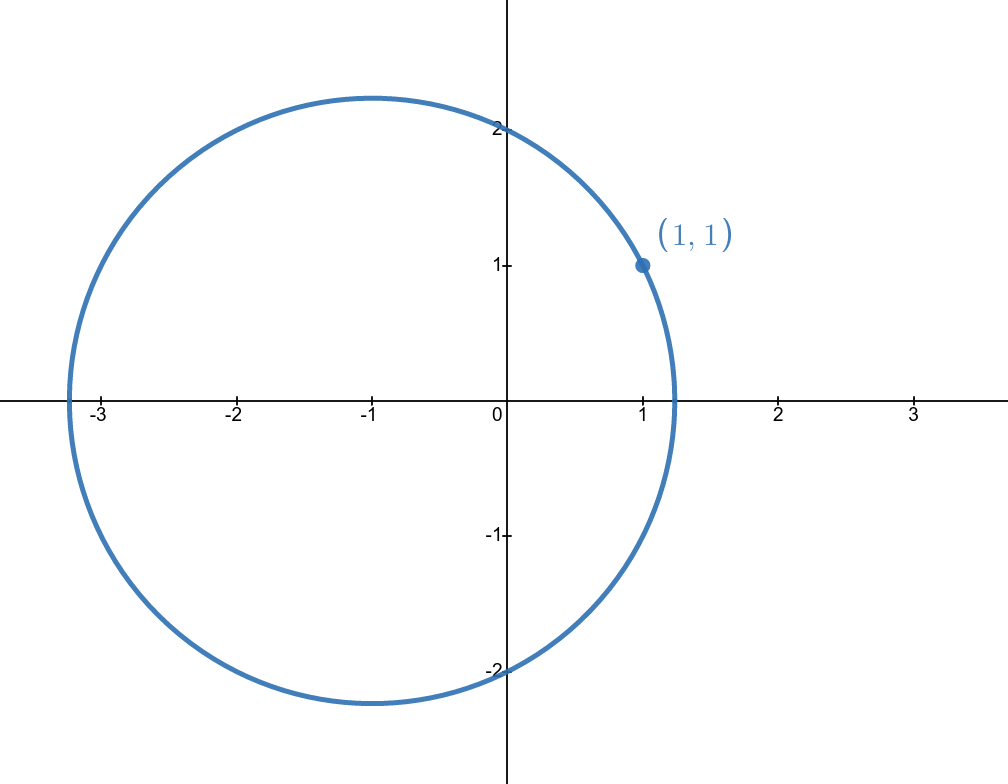
\includegraphics[scale=0.27]{cercle}
	\end{parts}

\end{questions}

\newpage
	
	\begin{Large}
	\textsc{Do not write on this page.}
	\end{Large}
	
	\vfill
	
	\textit{For officials use only:}
	\begin{center}
	\gradetable[h][questions]
	\end{center}
	
\end{document}